%%-*-latex-*-

% ------------------------------------------------------------------------
%
\begin{frame}
\frametitle{Trees}

Let us now present the concept of \textbf{tree}. A tree is either 
\begin{itemize}

  \item the empty set

  \item or a tuple made of a \textbf{root} and other trees, called
  \textbf{subtrees}.

\end{itemize}
This is a \textbf{recursive definition} because the object (here, the
tree) is defined by case and by grouping objects of the same kind
(here, the subtrees).

\bigskip

A root could be further refined as containing some specific
information.

\bigskip

It is usual to call \textbf{nodes} the root of a given tree and the
roots of all its subtrees, \emph{transitively}.

\bigskip

A node without non-empty subtrees is called a \textbf{leaf}.

\end{frame}

% ------------------------------------------------------------------------
%
\begin{frame}
\frametitle{Trees (cont)}

If we consider trees as relationships between nodes, it is usual to
call a root the \textbf{parent} of the roots of its direct subtrees
(i.e., the ones immediately in the tuple). Conversely, these roots are
\textbf{sons} of their parent (they are ordered).

\bigskip

It is also common to call subtree any tree included in it according to
the subset relationship (otherwise we speak of \emph{direct} subtrees).

\bigskip

Trees are often represented in a top-down way, the root being at the
top of the page, nodes as circles and the relationship between nodes
as \textbf{edges}. For instance:
\begin{center}
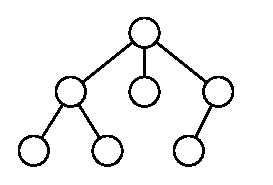
\includegraphics[bb=71 648 175 721]{tree_example}
\end{center}

\end{frame}

% ------------------------------------------------------------------------
%
\begin{frame}
\frametitle{Trees (cont)}

The \textbf{depth} of a node is the length of the path from the root
to it (note this path is unique). Thus the depth of the root is 0 and
the depth of the empty tree is undefined.

\bigskip

The \textbf{height} of a tree is the maximal depth of its nodes. For
example, the height of the tree in the previous page is 2.

\bigskip

A \textbf{level} in a tree is the set of all nodes with a given
depth. Hence it is possible to define level 0, level 1 etc. (may be
empty).

\end{frame}

% ------------------------------------------------------------------------
%
\begin{frame}
\frametitle{Trees/Traversals}

Given a tree, we can traverse it in many ways, but we must start from
the root since we do not have any other node at this level.

\bigskip

There are two main kind of traversals:
\begin{itemize}

  \item \textbf{Breadth-first} traversal consists in walking the
  tree by increasing levels: first the root (level 0), the sons of the
  root (level 1), then the sons of the sons (level 2) etc. 

  \item \textbf{Depth-first} traversal consists in walking the tree 
  by reaching the leaves as soon as possible.

\end{itemize}
In both cases, we are finished when all the leaves have been encountered.

\end{frame}

% ------------------------------------------------------------------------
%
\begin{frame}
\frametitle{Trees/Traversals/Breadth-first}

\label{breadth_first_pictures}

\begin{multicols}{2}
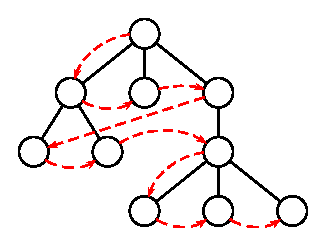
\includegraphics[bb=71 619 211 721]{breadth-first_1}

This is a \textbf{left to right} traversal.
\vfill\columnbreak
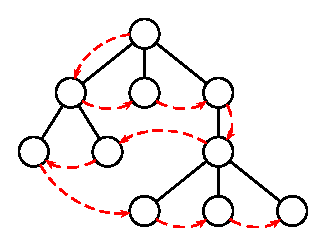
\includegraphics[bb=71 619 211 721]{breadth-first_2}
\end{multicols}
Many others are possible, like choosing randomly the next node of the
next level.

\end{frame}

% ------------------------------------------------------------------------
%
\begin{frame}
\frametitle{Trees/Traversals/Depth-first}

\begin{multicols}{2}
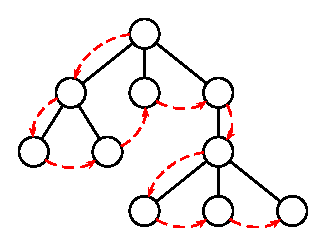
\includegraphics[bb=71 619 211 721]{depth-first_1}

This is a \textbf{left to right} traversal.

\vfill\columnbreak

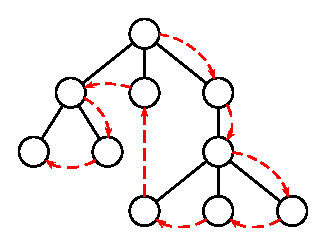
\includegraphics[bb=71 619 211 721]{depth-first_2}

This is a \textbf{right to left} traversal.

\end{multicols}

\end{frame}

% ------------------------------------------------------------------------
%
\begin{frame}
\frametitle{Trees/Binary trees}

Let us consider for a while binary trees only. Indeed, we do not lose
any generality with this apparent restriction because it is always
possible to map any tree to a binary tree in a unique way. One method
is the \textbf{left child/right sibling}:
\begin{center}
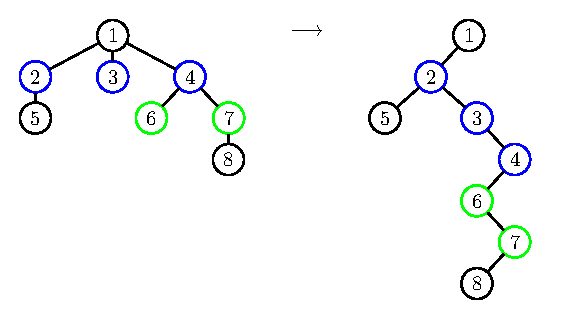
\includegraphics[bb=71 584 317 721]{left_brother}
\end{center}

\end{frame}

% ------------------------------------------------------------------------
%
\begin{frame}
\frametitle{Trees/Formal definition}

Let us formalise the concept of tree.
\begin{itemize}

  \item Let us note \proc{Empty} the empty tree. If the context is
    ambiguous, one can qualify the notation with the name of the data
    structure, for example, write \proc{Tree}.\proc{Empty} in order to
    make clear that we do not refer to empty stacks or empty queues.

  \item Let us note \(\proc{Join} (r, t_1, t_2)\) the tree whose
    root is \(r\), left subtree is \(t_1\) and right subtree is
    \(t_2\).
 
\end{itemize}

\end{frame}

% ------------------------------------------------------------------------
%
\begin{frame}
\frametitle{Trees/Examples}

Let us show some examples of tree construction:
\[\footnotesize
\begin{array}{c|c}
  \proc{Empty} 
& \varnothing\\
\hline
  \proc{Join} (\id{n_1}, \proc{Empty}, \proc{Empty})
& 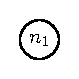
\includegraphics[bb=71 701 91 721]{n1}\\%[8pt]
\hline
  \proc{Join} (\id{n_1}, \proc{Empty}, \proc{Join} (\id{n_2},
  \proc{Empty}, \proc{Empty}))
& 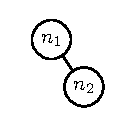
\includegraphics[bb=77 678 112 721]{n1_n2}\\%[10mm]
\hline
  \proc{Join} (\id{n_1}, \proc{Join} (\id{n_3},
  \proc{Empty}, \proc{Empty}), \proc{Join} (\id{n_2},
  \proc{Empty}, \proc{Empty}))
& 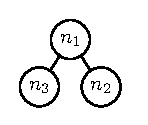
\includegraphics[bb=71 678 120 721]{n1_n2_n3}
\end{array}
\]

\end{frame}

% ------------------------------------------------------------------------
%
\begin{frame}
\frametitle{Trees/Basic projections}

Let us define the basic operations consisting in extracting the root,
the left subtree and the right subtree of a binary tree.
\begin{align*}
  \proc{Root} (\proc{Join} (r, t_1, t_2)) 
& \rightarrow r\\
  \proc{Left} (\proc{Join} (r, t_1, t_2))
& \rightarrow t_1\\
  \proc{Right} (\proc{Join} (r, t_1, t_2))
& \rightarrow t_2
\end{align*}
Note that these three operations are not defined on empty trees. In a
programming language, the case of the empty tree would be handled
explicitly, either by returning an error code (\C-like convention) or
throwing an exception (\Cpp like).

\bigskip

We also could specify the error situation in the rewrite system, as we
did for the division by zero, but we prefer not, in order to focus on
the concept, not the errors.

\end{frame}

% ------------------------------------------------------------------------
%
\begin{frame}
\frametitle{Trees/Left to right traversals}

\begin{multicols}{2}%[Consider a non-empty binary tree:]
\begin{center}
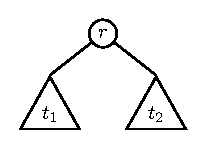
\includegraphics[bb=71 668 148 721]{non-empty_tree}
\end{center}

\vfill\columnbreak 

A depth-first traversal from left to right first visits node \(r\),
then the left subtree \(t_1\) and finally the right subtree
\(t_2\). But if we want to keep track of the visited nodes, we have
several ways.
\end{multicols}
\begin{itemize}

  \item We record \id{r}, then nodes of \id{t_1} and 
  nodes of \id{t_2}: this is \textbf{left prefix traversal};

  \item we record nodes of \id{t_1}, then \id{r} and nodes of
  \id{t_2}: this is a \textbf{left infix traversal}; 

  \item we record nodes of \id{t_1}, then nodes of \id{t_2} and
  \id{r}: this is a \textbf{left postfix traversal}.

\end{itemize}

\end{frame}

% ------------------------------------------------------------------------
%
\begin{frame}
\frametitle{Trees/Left-to-right prefix traversal}

In order to record the traversed nodes, we need an additional
structure: a stack.

\bigskip

The rewrite system corresponding to a left-to-right prefix traversal is
\begin{align*}
   \proc{Lpref} (\proc{Empty}) 
&  \rightarrow 
   \proc{Empty}\\
   \proc{Lpref} (\overline{\proc{Join} (\id{e}, \id{t_1}, \id{t_2})}) 
&  \rightarrow 
   \proc{Push} (\overline{\id{e}},
   \proc{Append} (\proc{Lpref} (\overline{\id{t_1}}), \proc{Lpref}
   (\overline{\id{t_2}})))
\end{align*}

\end{frame}

% ------------------------------------------------------------------------
%
\begin{frame}
\frametitle{Trees/Left-to-right postfix traversal}

The rewrite system corresponding to a left-to-right postfix traversal
is
\[
  \proc{Lpost} (\proc{Empty}) 
\rightarrow \proc{Empty}
\]
\begin{multline*}
  \proc{Lpost} (\overline{\proc{Join} (\id{e}, \id{t_1}, \id{t_2})}) 
\rightarrow\\
  \proc{Append} (\proc{Lpost} (\overline{\id{t_1}}),
     \proc{Append} (\proc{Lpost} (\overline{\id{t_2}}), 
                    \proc{Push} (\overline{\id{e}}, \proc{Empty})))
\end{multline*}

\end{frame}

% ------------------------------------------------------------------------
%
\begin{frame}
\frametitle{Trees/Left-to-right infix traversal}

The rewrite system corresponding to a left-to-right infix traversal is
\begin{align*}
   \proc{Linf} (\proc{Empty}) 
&\rightarrow \proc{Empty}\\
   \proc{Linf} (\proc{Join} (\id{e}, \id{t_1}, \id{t_2})) 
&\rightarrow \proc{Append} (\proc{Linf} (\id{t_1}), 
   \proc{Push} (\id{e}, \proc{Linf} (\id{t_2})))
\end{align*}

\end{frame}
